% Options for packages loaded elsewhere
\PassOptionsToPackage{unicode}{hyperref}
\PassOptionsToPackage{hyphens}{url}
\PassOptionsToPackage{dvipsnames,svgnames,x11names}{xcolor}
%
\documentclass[
  11pt,
]{book}
\title{Dispense sull'analisi delle componenti principali}
\usepackage{etoolbox}
\makeatletter
\providecommand{\subtitle}[1]{% add subtitle to \maketitle
  \apptocmd{\@title}{\par {\large #1 \par}}{}{}
}
\makeatother
\subtitle{Principal Component Analysis, PCA}
\author{Giorgio Marrubini e Camillo Melzi}
\date{}

\usepackage{amsmath,amssymb}
\usepackage{lmodern}
\usepackage{iftex}
\ifPDFTeX
  \usepackage[T1]{fontenc}
  \usepackage[utf8]{inputenc}
  \usepackage{textcomp} % provide euro and other symbols
\else % if luatex or xetex
  \usepackage{unicode-math}
  \defaultfontfeatures{Scale=MatchLowercase}
  \defaultfontfeatures[\rmfamily]{Ligatures=TeX,Scale=1}
\fi
% Use upquote if available, for straight quotes in verbatim environments
\IfFileExists{upquote.sty}{\usepackage{upquote}}{}
\IfFileExists{microtype.sty}{% use microtype if available
  \usepackage[]{microtype}
  \UseMicrotypeSet[protrusion]{basicmath} % disable protrusion for tt fonts
}{}
\makeatletter
\@ifundefined{KOMAClassName}{% if non-KOMA class
  \IfFileExists{parskip.sty}{%
    \usepackage{parskip}
  }{% else
    \setlength{\parindent}{0pt}
    \setlength{\parskip}{6pt plus 2pt minus 1pt}}
}{% if KOMA class
  \KOMAoptions{parskip=half}}
\makeatother
\usepackage{xcolor}
\IfFileExists{xurl.sty}{\usepackage{xurl}}{} % add URL line breaks if available
\IfFileExists{bookmark.sty}{\usepackage{bookmark}}{\usepackage{hyperref}}
\hypersetup{
  pdftitle={Dispense sull'analisi delle componenti principali},
  pdfauthor={Giorgio Marrubini e Camillo Melzi},
  colorlinks=true,
  linkcolor={Maroon},
  filecolor={Maroon},
  citecolor={Blue},
  urlcolor={Blue},
  pdfcreator={LaTeX via pandoc}}
\urlstyle{same} % disable monospaced font for URLs
\usepackage[left=2cm, right=2.5cm, top=2.5cm, bottom=2.5cm]{geometry}
\usepackage{color}
\usepackage{fancyvrb}
\newcommand{\VerbBar}{|}
\newcommand{\VERB}{\Verb[commandchars=\\\{\}]}
\DefineVerbatimEnvironment{Highlighting}{Verbatim}{commandchars=\\\{\}}
% Add ',fontsize=\small' for more characters per line
\usepackage{framed}
\definecolor{shadecolor}{RGB}{248,248,248}
\newenvironment{Shaded}{\begin{snugshade}}{\end{snugshade}}
\newcommand{\AlertTok}[1]{\textcolor[rgb]{0.94,0.16,0.16}{#1}}
\newcommand{\AnnotationTok}[1]{\textcolor[rgb]{0.56,0.35,0.01}{\textbf{\textit{#1}}}}
\newcommand{\AttributeTok}[1]{\textcolor[rgb]{0.77,0.63,0.00}{#1}}
\newcommand{\BaseNTok}[1]{\textcolor[rgb]{0.00,0.00,0.81}{#1}}
\newcommand{\BuiltInTok}[1]{#1}
\newcommand{\CharTok}[1]{\textcolor[rgb]{0.31,0.60,0.02}{#1}}
\newcommand{\CommentTok}[1]{\textcolor[rgb]{0.56,0.35,0.01}{\textit{#1}}}
\newcommand{\CommentVarTok}[1]{\textcolor[rgb]{0.56,0.35,0.01}{\textbf{\textit{#1}}}}
\newcommand{\ConstantTok}[1]{\textcolor[rgb]{0.00,0.00,0.00}{#1}}
\newcommand{\ControlFlowTok}[1]{\textcolor[rgb]{0.13,0.29,0.53}{\textbf{#1}}}
\newcommand{\DataTypeTok}[1]{\textcolor[rgb]{0.13,0.29,0.53}{#1}}
\newcommand{\DecValTok}[1]{\textcolor[rgb]{0.00,0.00,0.81}{#1}}
\newcommand{\DocumentationTok}[1]{\textcolor[rgb]{0.56,0.35,0.01}{\textbf{\textit{#1}}}}
\newcommand{\ErrorTok}[1]{\textcolor[rgb]{0.64,0.00,0.00}{\textbf{#1}}}
\newcommand{\ExtensionTok}[1]{#1}
\newcommand{\FloatTok}[1]{\textcolor[rgb]{0.00,0.00,0.81}{#1}}
\newcommand{\FunctionTok}[1]{\textcolor[rgb]{0.00,0.00,0.00}{#1}}
\newcommand{\ImportTok}[1]{#1}
\newcommand{\InformationTok}[1]{\textcolor[rgb]{0.56,0.35,0.01}{\textbf{\textit{#1}}}}
\newcommand{\KeywordTok}[1]{\textcolor[rgb]{0.13,0.29,0.53}{\textbf{#1}}}
\newcommand{\NormalTok}[1]{#1}
\newcommand{\OperatorTok}[1]{\textcolor[rgb]{0.81,0.36,0.00}{\textbf{#1}}}
\newcommand{\OtherTok}[1]{\textcolor[rgb]{0.56,0.35,0.01}{#1}}
\newcommand{\PreprocessorTok}[1]{\textcolor[rgb]{0.56,0.35,0.01}{\textit{#1}}}
\newcommand{\RegionMarkerTok}[1]{#1}
\newcommand{\SpecialCharTok}[1]{\textcolor[rgb]{0.00,0.00,0.00}{#1}}
\newcommand{\SpecialStringTok}[1]{\textcolor[rgb]{0.31,0.60,0.02}{#1}}
\newcommand{\StringTok}[1]{\textcolor[rgb]{0.31,0.60,0.02}{#1}}
\newcommand{\VariableTok}[1]{\textcolor[rgb]{0.00,0.00,0.00}{#1}}
\newcommand{\VerbatimStringTok}[1]{\textcolor[rgb]{0.31,0.60,0.02}{#1}}
\newcommand{\WarningTok}[1]{\textcolor[rgb]{0.56,0.35,0.01}{\textbf{\textit{#1}}}}
\usepackage{longtable,booktabs,array}
\usepackage{calc} % for calculating minipage widths
% Correct order of tables after \paragraph or \subparagraph
\usepackage{etoolbox}
\makeatletter
\patchcmd\longtable{\par}{\if@noskipsec\mbox{}\fi\par}{}{}
\makeatother
% Allow footnotes in longtable head/foot
\IfFileExists{footnotehyper.sty}{\usepackage{footnotehyper}}{\usepackage{footnote}}
\makesavenoteenv{longtable}
\usepackage{graphicx}
\makeatletter
\def\maxwidth{\ifdim\Gin@nat@width>\linewidth\linewidth\else\Gin@nat@width\fi}
\def\maxheight{\ifdim\Gin@nat@height>\textheight\textheight\else\Gin@nat@height\fi}
\makeatother
% Scale images if necessary, so that they will not overflow the page
% margins by default, and it is still possible to overwrite the defaults
% using explicit options in \includegraphics[width, height, ...]{}
\setkeys{Gin}{width=\maxwidth,height=\maxheight,keepaspectratio}
% Set default figure placement to htbp
\makeatletter
\def\fps@figure{htbp}
\makeatother
\setlength{\emergencystretch}{3em} % prevent overfull lines
\providecommand{\tightlist}{%
  \setlength{\itemsep}{0pt}\setlength{\parskip}{0pt}}
\setcounter{secnumdepth}{5}
\usepackage{booktabs}
\usepackage{amsmath}
\usepackage[italian]{babel}\addto\extrasitalian{
  \def\figureautorefname{Figura}
  \def\chapterautorefname{Capitolo}
  \def\sectionautorefname{Paragrafo}
  \def\subsectionautorefname{Paragrafo}
  \def\subsubsectionautorefname{Paragrafo}
  \def\equationautorefname{Equazione}
  \def\tableautorefname{Tabella}}
\usepackage{arydshln}
\ifLuaTeX
  \usepackage{selnolig}  % disable illegal ligatures
\fi
\usepackage[]{natbib}
\bibliographystyle{plainnat}

\begin{document}
\maketitle

{
\hypersetup{linkcolor=}
\setcounter{tocdepth}{1}
\tableofcontents
}
\hypertarget{section}{%
\chapter*{}\label{section}}
\addcontentsline{toc}{chapter}{}

\hypertarget{dati-multidimensionali}{%
\chapter{Dati multidimensionali}\label{dati-multidimensionali}}

\hypertarget{rappresentazione-matriciale-e-geometrica}{%
\section{Rappresentazione matriciale e geometrica}\label{rappresentazione-matriciale-e-geometrica}}

\begin{longtable}[]{@{}ccccc@{}}
\caption{\label{tab:RegrMult} Rappresentazione matriciale}\tabularnewline
\toprule
Indiv & \(X_1\) & \(X_2\) & \(\cdots\) & \(X_p\) \\
\midrule
\endfirsthead
\toprule
Indiv & \(X_1\) & \(X_2\) & \(\cdots\) & \(X_p\) \\
\midrule
\endhead
1 & \(x_{11}\) & \(x_{12}\) & \(\cdots\) & \(x_{m1}\) \\
2 & \(x_{21}\) & \(x_{22}\) & \(\cdots\) & \(x_{2p}\) \\
. & & & & \\
m & \(x_{1m}\) & \(x_{m2}\) & \(\cdots\) & \(x_{mp}\) \\
\bottomrule
\end{longtable}

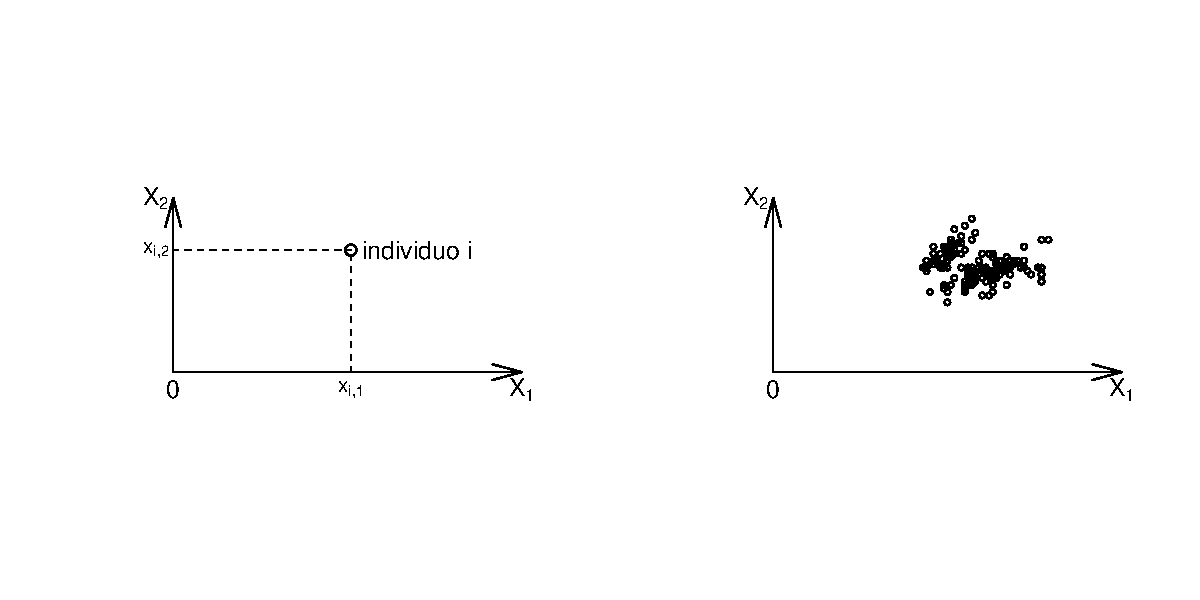
\includegraphics{dispense_pca_files/figure-latex/unnamed-chunk-1-1.pdf}

\hypertarget{trasformazione-delle-variabili-centratura-e-standardizzazione}{%
\section{Trasformazione delle variabili: centratura e standardizzazione}\label{trasformazione-delle-variabili-centratura-e-standardizzazione}}

Indichiamo con \(\bar{x_1},\dots,\bar{x_p}\) le medie delle variabili \(X_1,\dots,X_p\),
cioè le \(p\) medie delle \(p\) colonne della Tabella \ref{tab:RegrMult}, e con
\(\sigma_1^2,\dots,\sigma_p^2\) le rispettive varianze.\\
Il vettore \(\bar{x}=(\bar{x_1},\dots,\bar{x_p})\) viene chiamato \textbf{baricentro}.

\textbf{Centratura}: semplice traslazione del baricentro nell'origine
\begin{equation}
x_{ij}^{'}=x_{ij}-\bar{x_j}
\end{equation}

\begin{itemize}
\tightlist
\item
  non perdo informazione sulla distanza tra i punti (la geometria della nuvola di punti
  rimane invariata)
\item
  perdo solo informazione sul baricentro
\item
  semplifica formule e conti (da ora in poi useremo sempre dati centrati)
\end{itemize}

\textbf{Standardizzazione}: questa trasformazione porta ogni variabile ad avere varianza \(1\)
(in generale questa trasformazione viene fatta insieme alla centratura)
\begin{equation}
x_{ij}^{'}=\frac{x_{ij}-\bar{x_j}}{\sigma_j}
\end{equation}

\begin{itemize}
\tightlist
\item
  questa trasformazione rende le variabili degli scalari (numeri puri)
\item
  questa trasformazione è necessaria quando si vogliono confrontare variabili
  con differenti unità di misura (le variabili devono essere omogenee per essere confrontabili)
\item
  tutte le variabili hanno lo stesso ``peso''
\item
  cambia la distanza (la geometria) tra i punti. E' una dilatazione o contrazione.
\end{itemize}

Si veda la seguente figura per una rappresentazione grafica di dati centarti e
scalati per una matrice di dati di \(2\) variabili

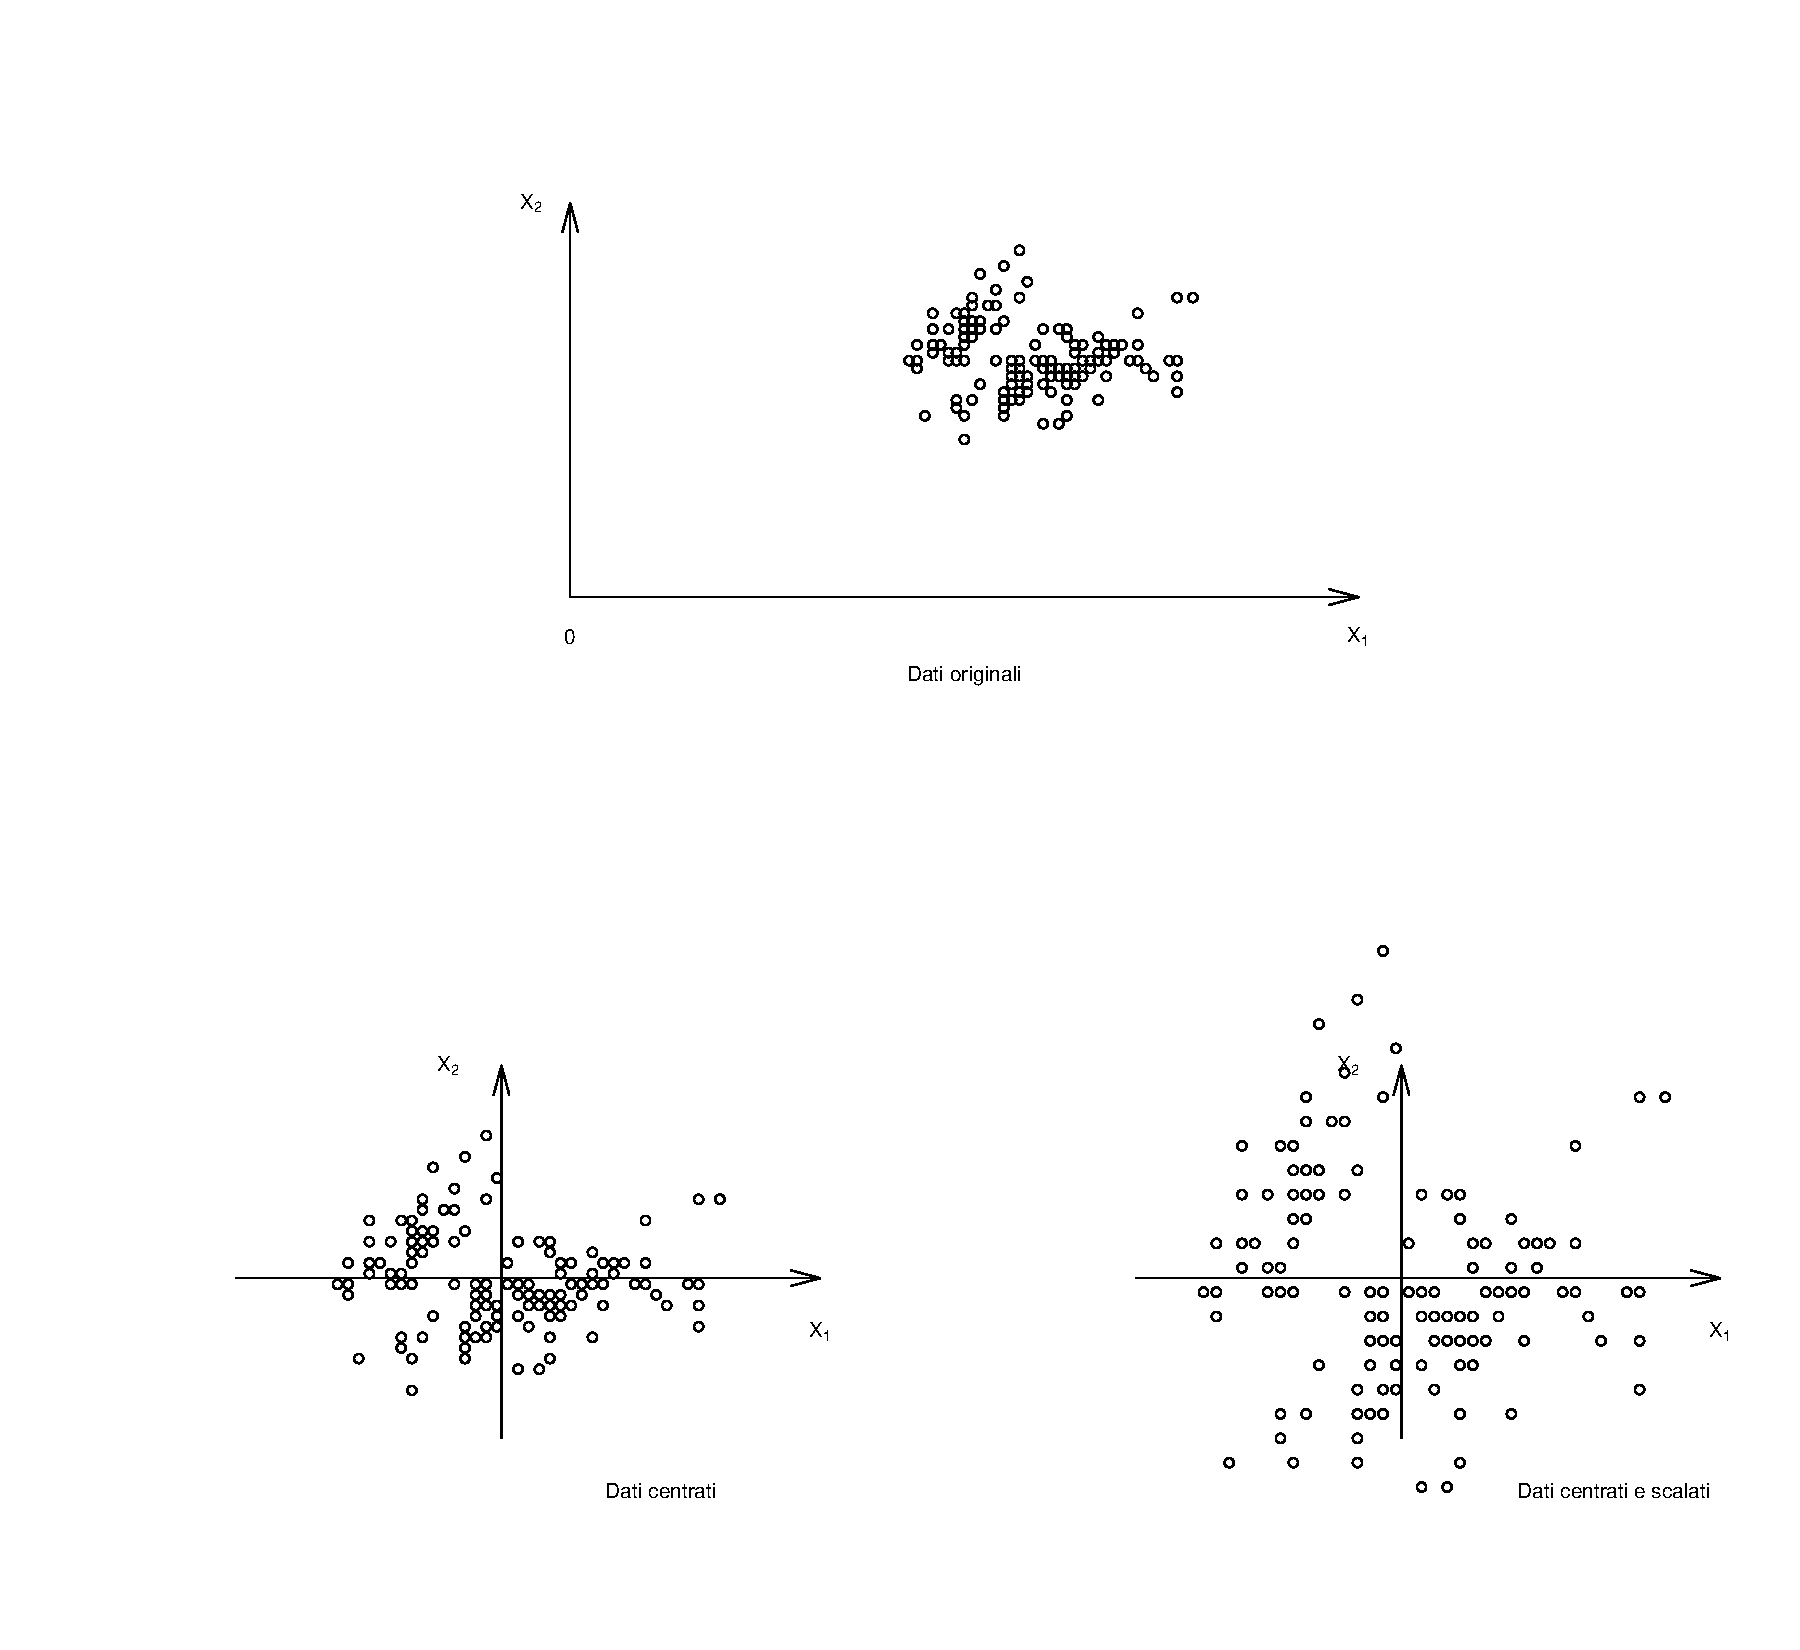
\includegraphics{dispense_pca_files/figure-latex/unnamed-chunk-2-1.pdf}

\hypertarget{matrice-di-covarianza-e-correlazione}{%
\section{Matrice di covarianza e correlazione}\label{matrice-di-covarianza-e-correlazione}}

\begin{equation}\label{eq:Cov}
Cov(X)=\left(
\begin{array}{cccc}
\sigma_{11}  & \dots & \sigma_{1p} \\
\vdots & \quad & \vdots \\
\sigma_{m1} & \dots & \sigma_{pp} \\
\end{array}
\right),
\end{equation}
dove \(\sigma_{ij}=\frac{1}{m-1}\sum_{k=1}^m(x_{ki}-\bar{x_i})(x_{kj}-\bar{x_j})\) è la covarianza tra
le variabili \(X_i\) e \(X_j\),
e in particolare\\
\(\sigma_{ii}=\sigma_i^2=\frac{1}{m-1}\sum_{k=1}^m(x_{ki}-\bar{x_i})^2\) è la varianza della variabile
\(X_i\).\\
Nel caso in cui i dati siano centrati \(Cov(X)=\frac{1}{m-1}X^tX\)

\begin{equation}\label{eq:Corr}
Cor(X)=\left(
\begin{array}{cccc}
1  & \dots & r_{1p} \\
\vdots & \quad & \vdots \\
r_{m1} & \dots & 1\\
\end{array}
\right),
\end{equation}

dove \(r_{ij}=\frac{\sigma_{ij}}{\sqrt{\sigma_{ii}\sigma_{jj}}}\) è la correlazione tra
le variabili \(X_i\) e \(X_j\).

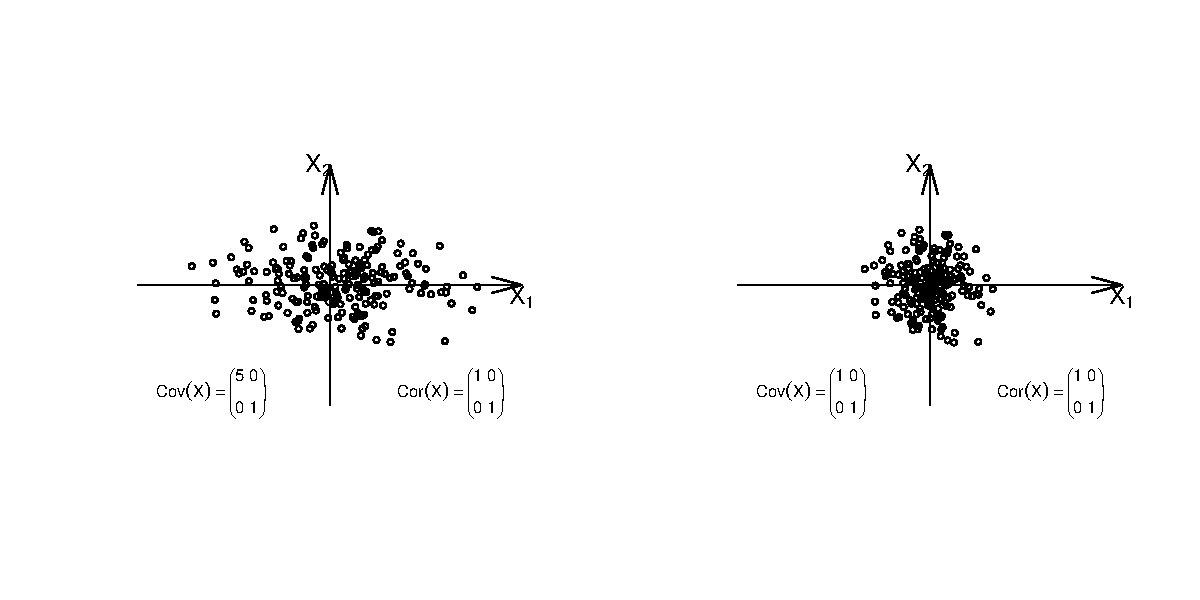
\includegraphics{dispense_pca_files/figure-latex/unnamed-chunk-3-1.pdf}

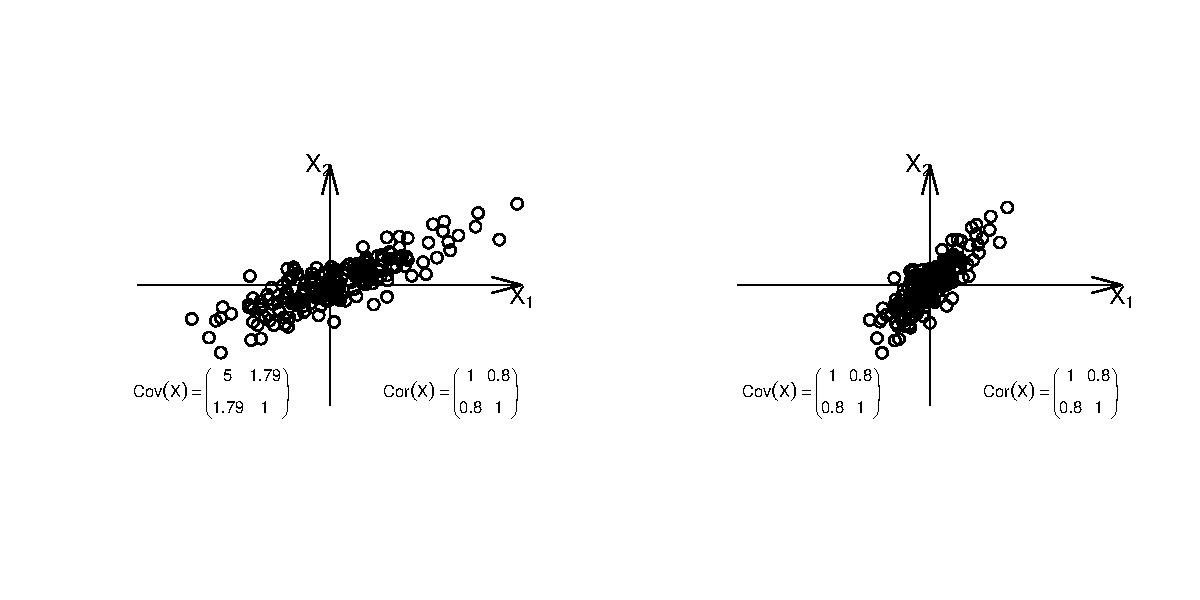
\includegraphics{dispense_pca_files/figure-latex/unnamed-chunk-4-1.pdf}

\hypertarget{variabili-latenti-o-componenti-e-proiezioni}{%
\section{\texorpdfstring{Variabili latenti o componenti e proiezioni \label{par:VariabiliLatenti}}{Variabili latenti o componenti e proiezioni }}\label{variabili-latenti-o-componenti-e-proiezioni}}

Sia \(T\) la combinazione lineare delle variabili \(X_1,\dots,X_p\), ossia il vettore
(si veda Figura \ref{fig:versore})
\begin{equation}
T=b_1X_1+\dots+b_pX_p,
\end{equation}
dove \(b_1^2+\dots+b_p^2=1\). Il vettore \(\textbf{b}=(b_1,\dots,b_p)\) è chiamato versore
e indica la direzione della variabile latente \(T\) (si veda Figura \ref{fig:versore}).

\begin{figure}
\centering
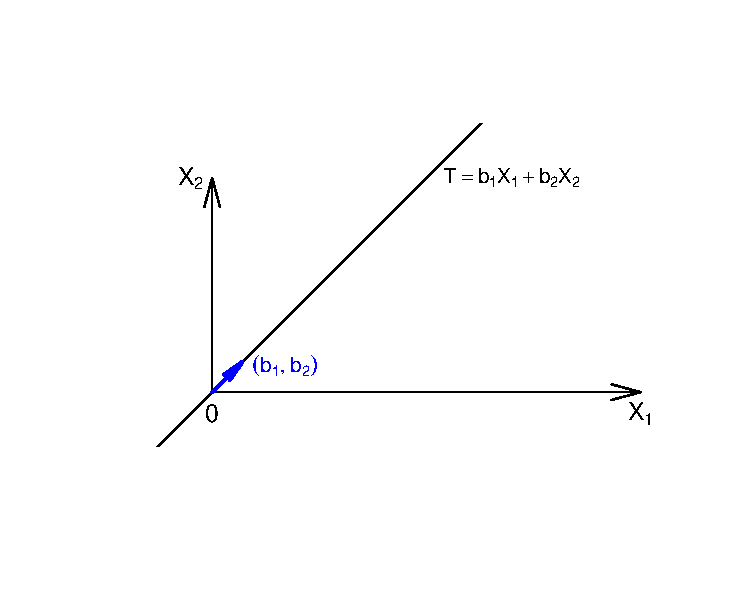
\includegraphics{dispense_pca_files/figure-latex/unnamed-chunk-5-1.pdf}
\caption{\label{fig:unnamed-chunk-5}Variabile latente \(T\)\label{fig:versore}}
\end{figure}

Sia \(\textbf{x}=(x_1,\dots,x_p)\) un generico punto (vettore) di \(\mathbf{R^p}\).
Chiamiamo proiezione di \(\textbf{x}\) su \(T\) il punto \(\textbf{x'}\) di \(T\) la
cui distanza da \(\textbf{x}\) è minima (si veda Figura \ref{fig:proiezione})

\begin{figure}
\centering
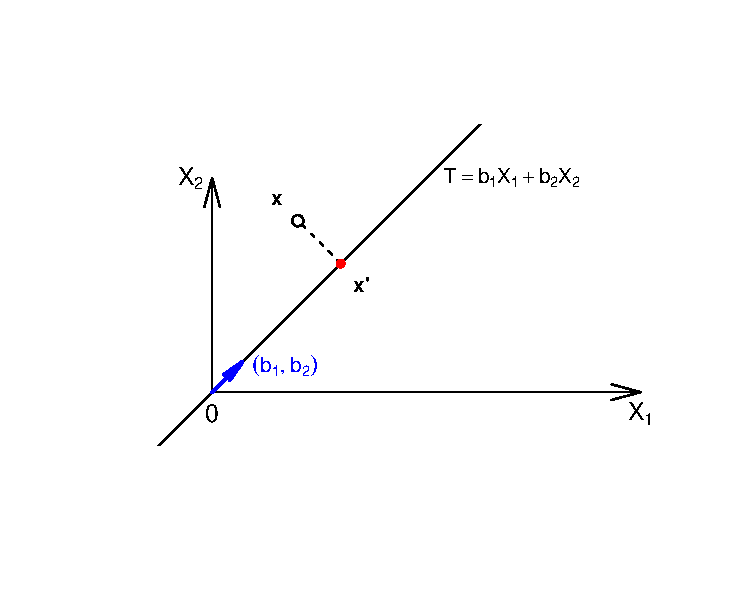
\includegraphics{dispense_pca_files/figure-latex/unnamed-chunk-6-1.pdf}
\caption{\label{fig:unnamed-chunk-6}Proiezione su \(T\)\label{fig:proiezione}}
\end{figure}

Definiamo \emph{componente} di \textbf{x} su T la lunghezza del vettore \(\|\textbf{x'} \|\) data da
\begin{equation}
\|\textbf{x'}\|=b_1x_1+\dots+b_px_p.
\end{equation}
I valori \(b_1,\dots,b_p\) sono chiamati \emph{loading} e la quantità
\(b_1x_1+\dots+b_px_p\) \emph{score}.

Si osservi che
\begin{equation}
\| \textbf{x'} \|=\|\textbf{x} \|\cos \theta
\end{equation}
ossia al prodotto interno (scalare) tra i vettori \(\textbf{x}\) e \(\textbf{b}\) (\(\| \textbf{b}\|=1\)).
Si veda la Figura \ref{fig:prodinterno}.

\begin{figure}
\centering
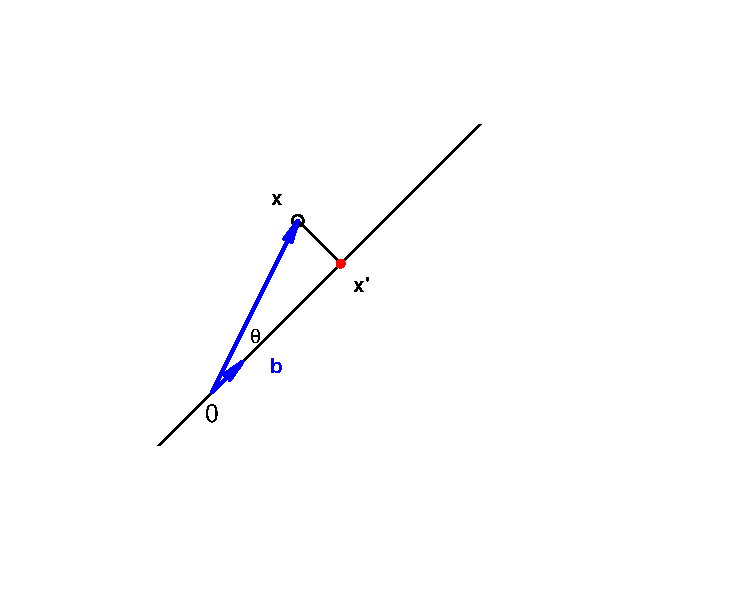
\includegraphics{dispense_pca_files/figure-latex/unnamed-chunk-7-1.pdf}
\caption{\label{fig:unnamed-chunk-7}Prodotto interno tra \textbf{x} e \textbf{b} \label{fig:prodinterno}}
\end{figure}

Proiezione degli \(m\) individui della matrice \textbf{X} sulla variabile latente T
\begin{equation}
\left(
\begin{array}{cccc}
x_{11}  & \dots & x_{1p} \\
\vdots & \quad & \vdots \\
x_{m1} & \dots & x_{mp} \\
\end{array}
\right)
\left(
\begin{array}{c}
b_1 \\
\vdots \\
b_m \\
\end{array}
\right)
=
\left(
\begin{array}{cccc}
b_1x_{11}  + \dots +b_p x_{1p} \\
\vdots   \\
b_1x_{m1} + \dots + b_px_{mp} \\
\end{array}
\right).
\end{equation}

Supponiamo di prendere una seconda variabile latente
\begin{equation}
T'=b'_1X_1+\dots+b'_pX_p, \qquad (b'_1)^2+\dots+(b'_p)^2=1
\end{equation}
e supponiamo che sia ortogonale a T (i.e \textbf{b} e \textbf{b'} ortogonali)
\begin{equation}
b_1b'_1+\dots+b_pb'_p=0.
\end{equation}
Si veda la Figura \ref{fig:proiezpiano}.

\begin{figure}
\centering
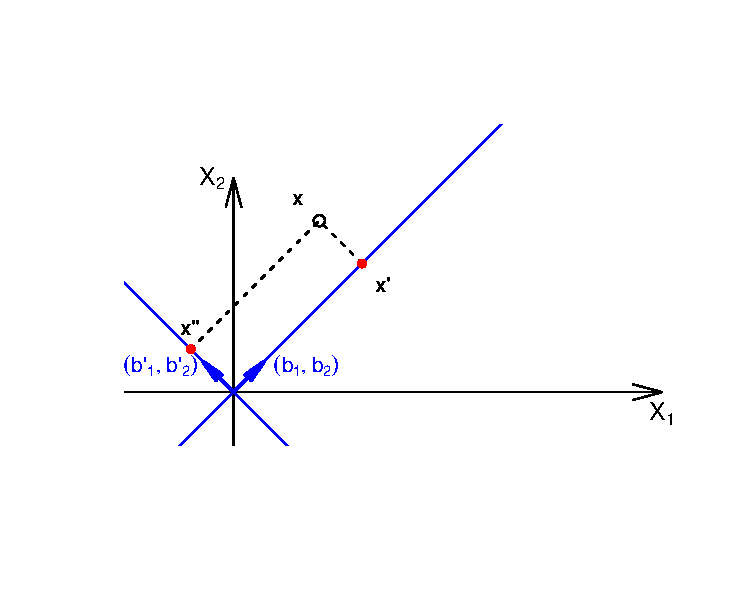
\includegraphics{dispense_pca_files/figure-latex/unnamed-chunk-8-1.pdf}
\caption{\label{fig:unnamed-chunk-8}Proiezione sul piano TT' \label{fig:proiezpiano}}
\end{figure}

Proiezione degli \(m\) individui della matrice \textbf{X} sul piano TT'
\begin{equation}
\left(
\begin{array}{cccc}
x_{11}  & \dots & x_{1p} \\
\vdots & \quad & \vdots \\
x_{m1} & \dots & x_{mp} \\
\end{array}
\right)
\left(
\begin{array}{cc}
b_1 & b'_1\\
\vdots & \vdots \\
b_m & b'_p\\
\end{array}
\right)
=
\left(
\begin{array}{cccc}
b_1x_{11}  + \dots +b_p x_{1p} & b'_1x_{11}  + \dots +b'_p x_{1p}\\
\vdots  & \vdots \\
b_1x_{m1} + \dots + b_px_{mp} & b'_1x_{m1} + \dots + b'_px_{mp} \\
\end{array}
\right).
\end{equation}

E' possibile iterare questo procedimento fino a p variabili latenti, in questo caso otteniamo
un cambio di basi (nuove coordinate). Abbiamo semplicemente ``cambiato prospettiva'' ruotando
il sistema di coordinate. Si veda la Figura \ref{fig:cambiobase}.

E' possibile fermarsi prima e proiettare su un
iperpiano,

Questo procedimento viene in generale eseguito perchè le variabili latenti
hanno certe proprietà desiderate.

Indicando con
\begin{equation}
P=
 \left(
 \begin{array}{cccc}
 b^1_1  & b^2_1 & \dots & b^p_1 \\
 \vdots &\vdots & \quad & \vdots \\
 b^2_m & b^2_m & \dots & b^p_m \\
 \end{array}
 \right) 
\end{equation}
la matrice dei \emph{loading}, si ha
\begin{equation}
 T=XP
\end{equation}
e ricordando l'ortonormalità dei vettori \(\textbf{b}_1,\dots,\textbf{b}_p\) (\(P^tP=I\))
\begin{equation}
 X=TP^t
\end{equation}

\begin{figure}
\centering
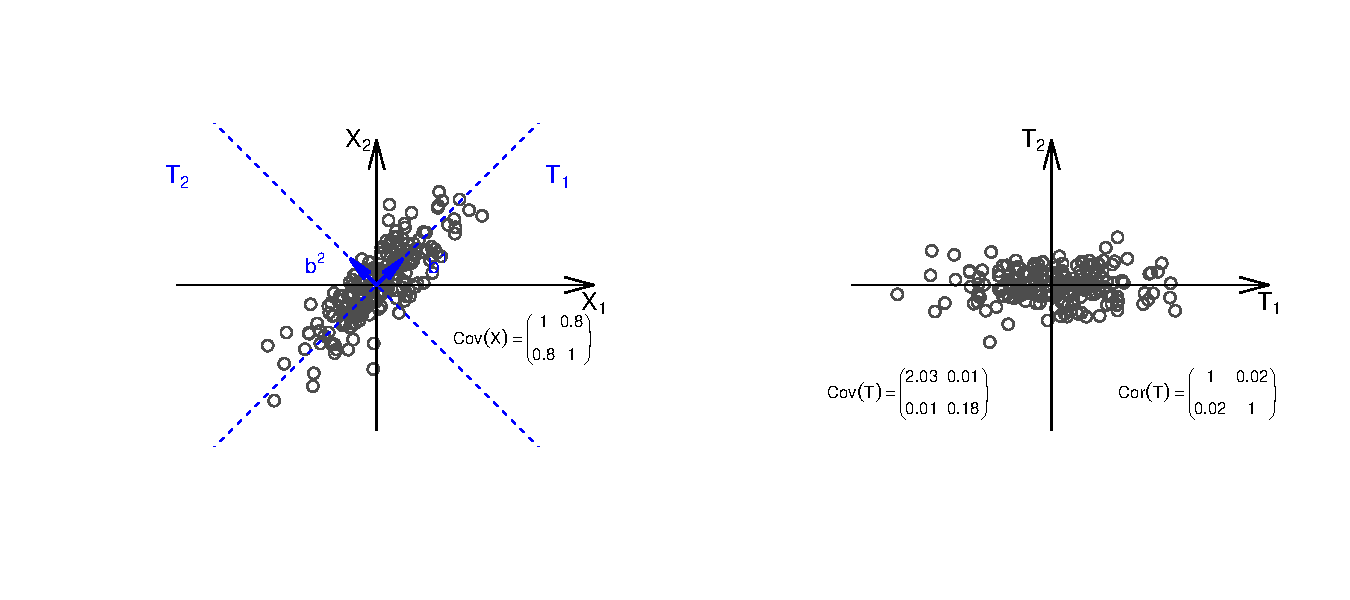
\includegraphics{dispense_pca_files/figure-latex/unnamed-chunk-9-1.pdf}
\caption{\label{fig:unnamed-chunk-9}Cambio base da \(X_1X_2\) a \(T_1T_2\) \label{fig:cambiobase}}
\end{figure}

\begin{Shaded}
\begin{Highlighting}[]
\NormalTok{P}\OtherTok{=}\FunctionTok{matrix}\NormalTok{(}\FunctionTok{c}\NormalTok{(}\DecValTok{1}\SpecialCharTok{/}\FunctionTok{sqrt}\NormalTok{(}\DecValTok{2}\NormalTok{),}\DecValTok{1}\SpecialCharTok{/}\FunctionTok{sqrt}\NormalTok{(}\DecValTok{2}\NormalTok{),}\SpecialCharTok{{-}}\DecValTok{1}\SpecialCharTok{/}\FunctionTok{sqrt}\NormalTok{(}\DecValTok{2}\NormalTok{),}\DecValTok{1}\SpecialCharTok{/}\FunctionTok{sqrt}\NormalTok{(}\DecValTok{2}\NormalTok{)),}\AttributeTok{ncol=}\DecValTok{2}\NormalTok{)}
\NormalTok{T}\OtherTok{=}\NormalTok{X}\SpecialCharTok{\%*\%}\NormalTok{P}
\FunctionTok{head}\NormalTok{(T)}
\end{Highlighting}
\end{Shaded}

\begin{verbatim}
##            [,1]         [,2]
## [1,] -0.8819306  0.469438535
## [2,] -1.1965330 -1.084705155
## [3,]  0.8871902  0.024327783
## [4,] -1.0638267  0.008888563
## [5,] -1.3798502 -0.102959280
## [6,] -1.3998573 -0.164815934
\end{verbatim}

\hypertarget{analisi-delle-componenti-principali}{%
\chapter{Analisi delle componenti principali}\label{analisi-delle-componenti-principali}}

Vogliamo costruire le variabili latenti \(T_1,\dots,T_p\) in modo da massimalizzare la distanza
tra gli \(m\) oggetti in \(\mathbb{R}^p\), le cui coordinate sono date dalla matrice \(X\) (cf.~),
nel senso che punti lontani in \(\mathbb{R}^p\) siano il più
lontano possibile nelle proiezioni su \(T_1\), poi \(T_2\),\ldots\ldots{}
La distanza tra i punti può essere misurata usando il teorema di Pitagora, distanza euclidea,
e questa è la formula della varianza delle variabili \(X_1,\dots,X_p\).\\
Vogliamo massimalizzare la varianza, perchè ad essa è associata l'informazione contenuta nei dati
in esame.
In definitiva vogliamo massimalizzare l'informazione ricavabile dagli oggetti in esama (varianza).

E' posssibile determinare una variabile latente \(T_1\), che chiameremo \emph{Prima Componente Principale},
in modo tale che

\begin{equation}
Var (T_1)=\rm{Max}_{\it{T}}\it{Var(T)}
\end{equation}
al variare di tutte le direzioni possibili \(T\) in \(\mathbb{R}^p\).\\
Tra tutte le variabili latenti perpendicolari alla \(T_1\) è possibile determinare una seconda
variabile latente \(T_2\), che chiameremo \emph{Seconda Componente Principale} in modo tale che

\begin{equation}
Var (T_2)=\rm{Max}_{\it{T\perp T_1}}\it{Var(T)}
\end{equation}

Questo procedimento può essere iterato fino alla costruzione di \(p\) componenti principali
\(T_1,T_2,\dots,T_p\).

Per quanto visto nel Paragrafo \ref{par:VariabiliLatenti} abbiamo determinato la matrice \(P\)
dei \emph{loading}. La matrice degli \emph{score} si ottiene
\begin{equation}\label{eq:Score}
T=XP
\end{equation}

La procedura per determinare \(P\) passa attraverso il calcolo degli autovalori
\(\lambda_1,\dots,\lambda_p\) della matrice di covarianza (di correlazione nel caso in cui i dati
fossero stati standardizzati)
\begin{equation}
Cov(X)=X^tX
\end{equation}

e dei relativi autovettori (le \(p\) componenti principali).

Uno dei risultati principali di questa costruzione è che nel sistema di coordinate delle componenti principali

\begin{equation}\label{eq:Corr_diag}
Cov(T)=\left(
\begin{array}{cccc}
\lambda_1  & \dots & 0 \\
\vdots & \quad & \vdots \\
0 & \dots & \lambda_m \\
\end{array}
\right),
\quad \lambda_1 \geq \lambda_2 \geq \dots \geq \lambda_m
\end{equation}

Conseguenze

\begin{itemize}
\tightlist
\item
  \(Var(T_i)=\lambda_i\)\\
\item
  varianza totale: \(\lambda_1+\dots+\lambda_p\)\\
\item
  le componenti \(T_1,T_2,\dots,T_p\) sono a indipendenti
\end{itemize}

  \bibliography{book.bib}

\addcontentsline{toc}{chapter}{Bibliografia}

\end{document}
